%======================================================================
\NEWSEC
%======================================================================

\subsection{\ssCharm}

\begin{frame}[fragile,label=ss-charm] 
\secframetitle{\ssCharm}
%--------------------------------------------------
\framesubtitle{MPI parallel programs: passing messages between processes}
%--------------------------------------------------
\begin{minipage}[t]{1.75in}
\begin{center}
\begin{minipage}{1.50in}
\includegraphics[width=1.50in]{mpi.pdf}\\
\vspace{-0.5in}
\centerline{\scriptsize\textbf{An MPI parallel program}}
\end{minipage}\\ \ \\
%\begin{minipage}{1.25in}
%\includegraphics[width=1.25in]{charm.pdf}
%\ \\
%\centerline{\scriptsize\textbf{A Charm\pp\ parallel program}}
%\end{minipage}
\end{center}
\end{minipage} \ 
\begin{minipage}[t]{2.50in}
\vspace{-0.6in}
\begin{itemize}
\item MPI program
  \begin{itemize}
  \item decomposed by \blueit{processes}
  \item calls MPI library
  \item communicate / synchronize
  \end{itemize}
\ \\ \pause
\item MPI runtime system
  \begin{itemize}
  \item sends data between processes
  \item synchronizes between processes
  \end{itemize} \pause
\item Additional features
\begin{itemize}
\item MPI-2: Parallel I/O, remote DMA,
one-sided communication
\item MPI-3: fault-tolerance, hybrid programming, persistence
\end{itemize}
\end{itemize}
\end{minipage}
\end{frame}

%----------------------------------------------------------------------

\begin{frame}[fragile]
\secframetitle{\ssCharm}
%--------------------------------------------------
\framesubtitle{\charm\ parallel programs: collections of asynchronously-interacting objects}
%--------------------------------------------------
\begin{minipage}[t]{1.75in}
\begin{center}
\begin{minipage}{1.25in}
\includegraphics[width=1.25in]{charm.pdf}
\ \\
\centerline{\scriptsize\textbf{A Charm\pp\ parallel program}}
\end{minipage}\\ \ \\
\ \\
\hrule
\ \\
\begin{minipage}{1.50in}
\includegraphics[width=1.50in]{mpi.pdf}\\
\vspace{-0.5in}
\centerline{\scriptsize{An MPI parallel program}}
\end{minipage}
\end{center}
\end{minipage} \ 
\begin{minipage}[t]{2.50in}
\vspace{-0.70in}
\begin{itemize}
\item \charm\ program
  \begin{itemize}
  \item Decomposed by \blueit{objects}
  \item \charm\ objects called \blueit{chares}
  \item invoke \blueit{entry methods}
  \item \blueit{asynchronous}
  \item communicate via \blueit{messages}
  \end{itemize}
\ \\ \pause
\item \charm\ runtime system
  \begin{itemize}
  \item maps chares to processors
  \item schedules entry methods
  \item migrates chares to load balance
  \end{itemize} \pause
\item Additional features
\begin{itemize}
\item checkpoint/restart
\item dynamic load balancing
\item fault-tolerance
\end{itemize}
\end{itemize}
\end{minipage}
\end{frame}

%----------------------------------------------------------------------
% \begin{frame}[fragile] 
% \secframetitle{\ssCharm}
%--------------------------------------------------
% \framesubtitle{Why use Charm++?}
%--------------------------------------------------
% \end{frame}
% ----------------------------------------------------------------------


\begin{frame}[fragile] 
\secframetitle{\ssCharm}
%--------------------------------------------------
%\framesubtitle{Anatomy of a simple Charm program}
%--------------------------------------------------

%     Look at simple HelloWorld Charm++ code
%        Control files
%          *.ci
         
%        Main
%        chare Group
%           one class created per process
% 	  indexed by ip
%        Chare Array
%           at least one class created per process

\begin{itemize}
\item C++ program with ``extra features''
\item Defined using ``\bluecode{.ci}'' control files: 
\begin{itemize}
\item which classes are chares
\item which methods are entry methods
\item declare message objects
\item declare global ``\code{readonly}'' variables
\end{itemize}
\item compiled using \bluecode{charmc}
\item generates \bluecode{.decl.h} and \bluecode{.def.h} from \bluecode{.ci}
\begin{itemize}
\item ``hooks'' program to \charm\ runtime
\item \bluecode{.decl.h} declarations
\item \bluecode{.def.h}: include definitions
\end{itemize}
\item Run executable using \bluecode{charmrun}
\end{itemize}
\end{frame}

% ----------------------------------------------------------------------
\begin{frame}[fragile] 
\secframetitle{\ssCharm}
\framesubtitle{Chare objects}
\framesubtitle{Chares are concurrent objects}
\begin{itemize}
\item Chares are C++ objects
\item Inherit from \charm\ base class
\footnotesize
\begin{semiverbatim}
#\bluetext{include} \orangetext{"foo.decl.h"}
\bluetext{class} \greentext{Foo} : \bluetext{public} \redtext{CBase_}\greentext{Foo} \{
   \bluetext{Foo} (\greentext{int} \orangetext{n});
   \greentext{void} \bluetext{p_receive_data} (\greentext{int} \orangetext{n}, \greentext{double} * \orangetext{a});
   \greentext{void} \bluetext{print_results} ();
\};
#\bluetext{include} \orangetext{"foo.def.h"}
\end{semiverbatim}
\normalsize
\item Chares and entry methods declared in \code{.ci} control file
\footnotesize
\begin{semiverbatim}
\greentext{module foo} \{
   \greentext{chare} \bluetext{Foo} \{
      \greentext{entry} \bluetext{Foo} (\greentext{int} \orangetext{n});
      \greentext{entry void} \bluetext{p_receive_data} (\greentext{int} \orangetext{n}, \greentext{double} \orangetext{a}[\orangetext{n}]);
   \};
\}
\end{semiverbatim}
\end{itemize}
%\normalsize
%\item \redcode{CBase\_}\greencode{Foo} declared in \bluecode{.decl.h} file
%\item \redcode{CBase\_}\greencode{Foo} defined in \bluecode{.def.h} file
%\end{itemize}
\end{frame}

% ----------------------------------------------------------------------
% \begin{frame}[fragile] 
% \secframetitle{\ssCharm}
% \framesubtitle{\charm\ control files}
% 
% \bluebf{Example control file: \bluecode{hello.ci}}
% 
%  \begin{semiverbatim}
%     \bluecode{mainmodule} \greencode{hello} \{
%        \bluecode{readonly} \greencode{CProxy_Main mainProxy};
%        \bluecode{mainchare} \greencode{main} \{
%           \bluecode{entry} \greencode{main}(\bluecode{CkArgMsg}*);
%        \};
%     \};
% \end{semiverbatim}
% \vspace{-0.2in}
% \begin{itemize}
% \item \charm\ programs start in a \blueit{mainchare}
% \item Other chares created dynamically using \bluecode{ckNew()}
% \begin{itemize}
% \item new chare may reside remotely
% \item \code{ckNew()} returns \blueit{proxy} to chare
% \item entry methods called via \bluetext{proxy}
% \end{itemize}
% 
% \end{itemize}
% \end{frame}

% ----------------------------------------------------------------------
\begin{frame}[fragile] 
\secframetitle{\ssCharm}
\framesubtitle{\charm\ collections of chares}
\vspace{-0.2in}
\begin{center}
\begin{minipage}{4in}
\begin{minipage}{1.5in}
\bluebf{Chare Arrays}
\end{minipage} \ 
\begin{minipage}{2in}
\includegraphics[width=2.0in]{chare-array.pdf}
\end{minipage}
\vspace{0.1in}
  \begin{itemize}
  \item \bluetext{distributed array of chares}
  \item \bluetext{migratable elements}
  \item \bluetext{flexible indexing}
  \end{itemize}
\vspace{0.2in}
\begin{minipage}{1.5in}
\redbf{Chare Groups}
\end{minipage} \ 
\begin{minipage}{2in}
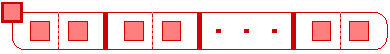
\includegraphics[width=2.0in]{chare-group.pdf}
\end{minipage}
  \begin{itemize}
\setbeamercolor*{item}{fg=red!50!black}
  \item \redtext{one chare per processor (non-migratable)}
  \end{itemize}
\vspace{0.2in}
\begin{minipage}{1.5in}
\greenbf{Chare Nodegroups}
\end{minipage} \ 
\begin{minipage}{2in}
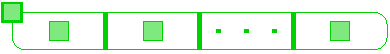
\includegraphics[width=2.0in]{chare-nodegroup.pdf}
\end{minipage}
  \begin{itemize}
\setbeamercolor*{item}{fg=green!50!black}
  \item \greentext{one chare per node (non-migratable)}
  \end{itemize}
\end{minipage}
\end{center}

\end{frame}
